\documentclass[conference]{IEEEtran}
\IEEEoverridecommandlockouts

\usepackage{cite}
\usepackage{amsmath,amssymb,amsfonts}
\usepackage{graphicx}
\usepackage[caption=false,font=footnotesize]{subfig}
\usepackage{textcomp}
\usepackage{xcolor}
\usepackage{booktabs}
\usepackage{hyperref}

\setlength{\textfloatsep}{6pt}
\setlength{\floatsep}{5pt}

\begin{document}

\title{Behavioral Stability of Quantized Large Language Models Under Prompt Drift: The Resilio Evaluation Framework}

\author{
\IEEEauthorblockN{Vedant Barhate}
\IEEEauthorblockA{
\textit{School of Computing} \\
\textit{MIT ADT University} \\
Pune, India \\
vedant.barhate27@gmail.com}
\and
\IEEEauthorblockN{Yash Pandey}
\IEEEauthorblockA{
\textit{School of Computing} \\
\textit{MIT ADT University} \\
Pune, India \\
pandeyyash25@gmail.com}
\and
\IEEEauthorblockN{Achyut Yesare}
\IEEEauthorblockA{
\textit{School of Computing} \\
\textit{MIT ADT University} \\
Pune, India \\
achyutyesare886@gmail.com}
\and
\IEEEauthorblockN{Vibhor Dev}
\IEEEauthorblockA{
\textit{School of Computing} \\
\textit{MIT ADT University} \\
Pune, India \\
vibhor.101605@gmail.com}
}

\maketitle

\begin{abstract}
Large Language Models are increasingly deployed using quantization techniques such as 8-bit and 4-bit precision to reduce memory footprint and inference costs. While these models perform well on clean benchmarks, real-world deployment encounters ``Prompt Drift''---typographical errors, informal phrasing, and structural degradation.

Studying the link between model quantizing and five incremental tiers of prompt quality decline across Llama 3.1 8B, Mistral 7B, and Phi-3 Mini, Resilio is a methodical evaluation tool. Two measures we use to evaluate behavioral stability are the Behavioral Stability Score (BSS) and the Task Performance Score (TPS).

Our close analysis of 5,760 model responses shows that modern quantization approaches create virtually little additional deterioration over the main drift effect. Four-bit quantization merely makes the system 1–3% less stable in every tested configuration compared to FP16 benchmarks. On the other hand, just by quick drift, the system becomes 15-35% less stable. Still, there are activity-specific patterns: Tasks requiring a lot of thinking depend on quantization a little bit more than do classification initiatives.

These findings challenge assumptions about quantized model frailty and suggest that, for most real world applications, deployment decisions should prioritize model architecture choice and input quality control over quantization level selection.
\end{abstract}

\begin{IEEEkeywords}
Quantization, Large Language Models, Prompt Drift, Behavioral Stability, BSS, TPS, Robustness, Deployment
\end{IEEEkeywords}

\section{Introduction}

Because of the need for lower latency, better privacy, and lower operational costs, Large Language Models are  being started used in edge environments with a limited resources instead of centralized data centers. The standard way to optimize  is now Post-training quantization , and it  does reduces model weights from 16-bit floating point (FP16) to 8-bit or 4-bit precision. These methods compress memory a lot without affecting the accuracy of clean input too much, but we still don't know how they work when the input gets worse in real life.

\subsection{The Phenomenon of Prompt Drift}

Using ``ideal'' benchmarks distinguished by well-structured syntax, standard evaluation procedures assesses LLMs. Production settings expose models to a continuous input degradation, a phenomena we formalize as textit{Prompt Drift}. Prompt drift is the inherently present noise in human-AI interaction across five degrees of severity:

\begin{itemize}
\item \textbf{L1 – Typographical Noise:} Introduction of character-level errors such as misspellings, adjacency mistakes, and letter transpositions while preserving overall structure and meaning.
    
\item \textbf{L2 – Formatting Loss:} Removal of capitalization, punctuation, and standard formatting cues, leading to reduced structural clarity without altering core semantics.

\item \textbf{L3 – Linguistic Informality:} Incorporation of slang, abbreviations, and colloquial expressions (e.g., ``u'', ``pls'', ``bc''), introducing deviations from formal language patterns.

\item \textbf{L4 – Structural Degradation:} Breakdown of grammatical structure through word merging, spacing errors, and syntactic inconsistencies that affect sentence readability.

\item \textbf{L5 – Semantic Fragmentation:} Severe degradation characterized by incomplete phrases, truncated context, and fragmented instructions, leading to partial or ambiguous semantic representation.
\end{itemize}

\subsection{The Critical Evaluation Gap}

One of the most basic issues in deployed artificial intelligence concerns the interplay between quantization and genuine input degradation. Using clear benchmarks and robustness through full-precision models, earlier studies evaluate quantization; therefore, there is a serious dearth of measurements on their interaction. Two opposing theories exist: quantization
 might improve sensitivity to input noise by reducing numerical accuracy; alternatively, contemporary compression techniques could be effective enough that the results of quantization are minor relative to the effects of drift.

By methodically contrasting model families, quantization levels, task groups, and drift degrees, the \textit{Resilio} framework answers this issue. Employing multi-dimensional stability scoring gives us real-world data on interaction between quantization and drift, which informs our deployment decisions.

\section{Related Work}

The quest of deploying Large Language Models (LLMs) on edge devices has created research into two previously distinct domains: computational optimization through quantization and the linguistic robustness of models under disturbance. The \textit{Resilio} framework operates at the intersection of these fields.

\subsection{LLM Quantization for Efficient Deployment}

The need for on-device LLM execution has led to the rapid exploration of Post-Training Quantization (PTQ) techniques. As noted by Dettmers \textit{et al.}~\cite{ref1}, 8-bit matrix multiplication allows for significant memory reduction with negligible or minimal performance loss on standard benchmarks. The introduction of 4-bit quantization further pushes these boundaries, allowing models like Phi-3, Llama 3.1, and Mistral 7B to operate within the strict memory constraints of mobile hardware~\cite{ref2, ref3, ref19}. 

However, while prior studies provide good evaluation of the resource efficiency of INT4 versus INT8 representations~\cite{ref14, ref18}, these studies typically is based on ``clean'' input distributions. Recent work suggests that such extreme compression levels may introduce hidden instabilities or alter model safety alignment—a phenomenon sometimes termed \textit{quantization-based vulnerability}~\cite{ref10, ref13}.

\subsection{Robustness to Input Perturbations and Prompt Drift}

The sensitivity of LLMs to surface-level changes in input text is a highly explored challenge. Research into typographical noise~\cite{ref12} and naturally occurring errors in training data~\cite{ref9} confirms that even slight character-level deviations often produces significant variance in model output. Frameworks such as PromptBench have begun to standardize the measurement of model resilience against adversarial attacks~\cite{ref5, ref21}. 

Furthermore, studies on ``noisy instructions'' indicate that the quality of the prompt is a primary determinant of zero-shot generalization~\cite{ref11}. Despite these insights, existing robustness studies primarily utilize full-precision (FP16 or FP32) models only, leaving the stability of quantized models under similar \textit{Prompt Drift} largely unmeasured~\cite{ref4}.

\subsection{Behavioral Stability and Runtime Monitoring}

As AI agents move into production, \textit{behavioral stability} has emerged as a more than simple accuracy. This stability can be defined as the consistency of model behavior across prompt variations~\cite{ref6}. In real-world deployments, \textit{data drift}—the shift in the distribution of user inputs over time—presents a constant risk to model reliability and behavior.~\cite{ref7}. 

While researchers have proposed various runtime monitoring strategies to detect behavioral shifts in AI systems~\cite{ref20}, there is no unified metrics that measure stability relative to a clean baseline. The interaction between acceleration techniques and these hidden instabilities remains an open area of research~\cite{ref13}.

\subsection{Identification of Research Gaps}

A systematic review of the literature reveals a critical three--part gap:

\begin{itemize}
\item \textbf{Isolation of Factors:} Quantization is typically evaluated on clean inputs, while robustness is tested on full-precision models. The interaction between bit-precision and input drift is largely omitted.

\item \textbf{Absence of Graduated Drift Frameworks:} Most studies rely on binary noise conditions (clean vs.\ noisy) rather than a structured, multi-level taxonomy (L1--L5) as proposed in this work.

\item \textbf{Metric Limitations:} Standard accuracy metrics fail to capture \textit{silent failures}, where a model maintains high confidence despite producing logically inconsistent or incorrect outputs.
\end{itemize}

By introducing the \textit{Task Performance Score (TPS)} and \textit{Behavioral Stability Score (BSS)}, the \textit{Resilio} framework provides a multi-factor analysis of task-specific stability patterns under quantization and prompt drift.

\section{The Resilio Methodology}

The \textit{Resilio} framework's architecture is based on a modular, repeatable pipeline that connects synthetic benchmarks with the random nature of noise in production-level input. The method is carried out in three steps: creating a custom dataset, simulating object-oriented drift, and checking for semantic correctness.

\subsection{Dataset Architecture}

To enable a detailed examination of model stability, we assembled a specialized dataset consisting of 40 foundational prompts. These prompts are organized in a way that makes them look like common language problems, but they were made to focus on specific behavioral limits in Large Language Models:

\begin{itemize}
\item \textbf{Reasoning:} 10 prompts engineered to evaluate multi-step mathematical logic and sequential deduction.
\item \textbf{Logical Inference:} 10 prompts structured to assess complex deductive reasoning and syllogistic consistency.
\item \textbf{Question Answering:} 10 prompts focused on the precision of factual retrieval and context-window utilization.
\item \textbf{Sentiment Classification:} 10 prompts designed to measure the robustness of pattern recognition under lexical noise.
\end{itemize}

\subsection{OOP-based Drift Generation Framework}

The heart of Resilio is a drift generator that uses Object-Oriented Programming (OOP). This modular engine lets you use graduated, additive transformations that mimic realistic user-driven degradation. To make sure that the results were statistically diverse, each base prompt was given 16 different variations.

The framework formalizes \textit{Prompt Drift} into a five-tier severity taxonomy:

\begin{itemize}
\item \textbf{L1 (Character-level Perturbation):} Simulates typographical errors via keyboard adjacency mapping and character transpositions.
\item \textbf{L2 (Form Degradation):} Implements systematic removal of casing, standard punctuation, and formal whitespace.
\item \textbf{L3 (Linguistic Shift):} Replaces formal lexical units with slang, non-standard abbreviations, and colloquial expressions.
\item \textbf{L4 (Grammatical Breakdown):} Induces word merging, omission of essential function words, and overall syntactic collapse.
\item \textbf{L5 (Structural Truncation):} Combines aggressive informality with content reduction, forcing the model to infer intent from fragmented inputs.
\end{itemize}

\subsection{Mathematical Validation of Realism}

We use the \texttt{all-MiniLM-L6-v2} SentenceTransformer model to check the quality of the perturbations mathematically. This makes sure that the drift we create is realistic "noisy" input and not just random gibberish. We find the cosine similarity between the clean baseline (L0) and each variant that has drifted.

Formally, for embedding vectors $\mathbf{u}$ (clean prompt) and $\mathbf{v}$ (drifted prompt), cosine similarity is defined as:

\begin{equation}
\text{CosineSimilarity}(\mathbf{u}, \mathbf{v}) =
\frac{\mathbf{u} \cdot \mathbf{v}}{\|\mathbf{u}\| \, \|\mathbf{v}\|}
\end{equation}

The generated variants are required to satisfy strict semantic similarity ranges:

\begin{itemize}
\item \textbf{L1:} 93.2\% similarity (high surface-level fidelity)
\item \textbf{L2:} 88.1\% similarity (loss of structural metadata)
\item \textbf{L3:} 83.4\% similarity (lexical divergence)
\item \textbf{L4:} 77.8\% similarity (syntactic fragmentation)
\item \textbf{L5:} 71.5\% similarity (boundary of semantic coherence)
\end{itemize}

This metric confirms that the \textit{Resilio} framework provides a precisely controlled and semantically grounded stress test for evaluating quantized language model behavior.

\section{Metric Formulation (TPS \& BSS)}

The main analytical innovation of the \textit{Resilio} framework is moving beyond simple accuracy metrics to a comprehensive evaluation of model reliability. By separating performance focus from structural consistency, it introduces a dual-metric approach that effectively looks after the detailed performance degradation in quantized LLMs.

\subsection{Task Performance Score (TPS): The 5-Factor Behavioral Matrix}

Traditional benchmarking often fails to identify ``silent failures''—instances where a model maintains linguistic fluency while undergoing logical or factual collapse or degradation. To quantify these effects, each response is evaluated across a weighted five-dimensional behavioral vector:

Standard benchmarking frequently does not detect ``silent failures`` which are situations in which a model preserves linguistic fluency while experiencing logical or factual or reasoning drop. To measure these effects, each response is rated on a five-dimensional behavioural vector with different weights:

\begin{itemize}
\item \textbf{Factual Correctness (FC):} Cross-referencing the model’s terminal output against ground-truth metadata.
\item \textbf{Logical Correctness (LC):} Verification of deductive validity and mathematical accuracy of intermediate steps.
\item \textbf{Reasoning Coherence (RC):} Assessment of structural integrity and sequential clarity of the explanation.
\item \textbf{Sentiment Correctness (SC):} Evaluation of label accuracy for pattern-matching and classification tasks.
\item \textbf{Manner of Language (ML):} A calibration metric measuring whether linguistic confidence aligns with actual output accuracy.
\end{itemize}

The Task Performance Score (TPS) is computed as:

\begin{equation}
TPS = \sum_{i=1}^{5} \left( w_i \cdot \text{Score}_i \right)
\end{equation}

where $w_i$ denotes task-specific weight coefficients. These weights are dynamically adjusted; for example, Logical Correctness ($LC$) is prioritized in reasoning tasks, while Sentiment Correctness ($SC$) is stressed in classification settings.

\subsection{Behavioral Stability Score (BSS)}

The \textit{Behavioral Stability Score (BSS)} measures how well a model can handle input degradation, while TPS measures its overall performance. BSS gives a relative stability index that does not depend on the size of the model by normalising degraded performance against a clean base.

For a given drift level $d$, BSS is defined as:

\begin{equation}
BSS_d = \frac{\overline{TPS}_d}{TPS_0}
\end{equation}

where $\overline{TPS}_d$ represents the mean Task Performance Score across all variants at drift level $d$, and $TPS_0$ denotes performance on the clean baseline (L0).

\subsection{Stability Threshold and Behavioral Collapse}

A primary empirical finding of this study is the establishment of a stability threshold characterised by $BSS < 0.7$. This line separates "safe degradation" from "behavioural collapse."

The 0.7 threshold was chosen because it shows a difference between being fluent in a language and being factually correct. When the threshold is lower, "silent failures" happen more often. This means that models keep high Manner of Language ($ML$) scores while their Factual Correctness ($FC$) and Logical Correctness ($LC$) scores go down a lot.

The \textit{Resilio} framework makes this threshold official, which gives us a useful safety measure for figuring out what quantization levels are okay to use in real-world deployment situations.


\section{Experimental Setup and Implementation}

The empirical validation of the \textit{Resilio} framework utilised a large-scale, multi-threaded computational pipeline aimed at quantifying the convergence of model architecture, bit-precision depth, and input degradation. The implementation was designed to make sure that all test configurations had the same environmental conditions so that the effects of quantisation and drift could be studied separately.
\subsection{Technical Infrastructure and Model Configurations}

For precise management, the research made use of a high-performance computer setup based on the textit{Hugging Face} ecosystem and the textit{BitsAndBytes} library. Three open-source models with varied parametric scales and architecture were selected: \textit{Llama 3.1 8B}, \textit{Mistral 7B}, and \textit{Phi-3 Mini}. Each model was instantiated in three different quantisation variants:

\begin{itemize}
\item \textbf{FP16:} The 16-bit floating-point baseline.
\item \textbf{INT8:} 8-bit quantization using vector-wise quantization logic.
\item \textbf{INT4:} 4-bit quantization with double quantization enabled for maximum memory efficiency.
\end{itemize}

To maintain internal validity, we enforced consistent generation parameters across all 5,760 total inferences, utilizing a temperature of 0.7, a top-$p$ value of 0.9, and a maximum token limit of 350.

\subsection{The LLM-as-Judge Evaluation Pipeline}

We found that manually annotating 5,760 multi-factor responses was not possible, so we created an automated evaluation pipeline that used \textit{GPT-OSS 20B} as a neural rater and could be accessed through the \textit{Groq API}. The structured JSON protocol that this LLM-as-Judge system was given told it to find a five-dimensional scoring vector for each response. The five dimensions were Factual Correctness (FC), Logical Correctness (LC), Reasoning Coherence (RC), Sentiment Correctness (SC), and Manner of Language (ML).

To resolve  this technical bottlenecks and to ensure data integrity, this  pipeline implemented:

\begin{itemize}\item \textbf{Asynchronous Threading:} Designed to maintain an optimal throughput of 30 requests per minute (RPM) and it should  manage API rate limits during the  inference.
\item \textbf{Contextual Grounding:} Each evaluation request included the original clean prompt and The  ground-truth metadata for  preventing  evaluators hallucination.
\item \textbf{Memory Management:} Automated GPU offloading and memory cleaning were utilized between quantization cycles to prevent VRAM fragmentation during local INT4/INT8 testing.
\end{itemize}
\subsection{TPS and BSS Computation \& Visualization}

After the evaluation phase, the extracted scoring vectors were combined to get the main metrics: the Task Performance Score (TPS) and the Behavioral Stability Score (BSS). The TPS for each individual response was calculated using a weighted combination of the five evaluation factors. The weights were specific to each category to account for the different needs of Reasoning, Logic, Question Answering, and Classification tasks.

Later, the Behavioral Stability Score (BSS) was calculated for each drift level as the ratio of the mean TPS of degraded prompt variants ($\overline{TPS}_d$) to the TPS of the corresponding clean baseline ($TPS_0$). This normalization made it possible to directly compare degradation trajectories to ideal conditions, regardless of the scale of the model.

The results were organized by model architecture, quantization level, task category, and drift level so that they could be analyzed in much detail. To find The  degradation trends and amplification effects caused by quantization, here we used visualization Methods like line plots for BSS trajectories, bar charts for prompt-level variation, and heatmaps for  the category-wise stability patterns.

This multi-level visualization framework make it easy for  understanding that  how behavior changed in all of the experiments.

This multi-level visualization framework made it easy to understand how behavior changed in all of the experiments.


\section{Results, Analysis, and Discussion}

% --- FIGURE 1: FULL WIDTH (INTRO CONTEXT) ---
\begin{figure*}[t]
\centering
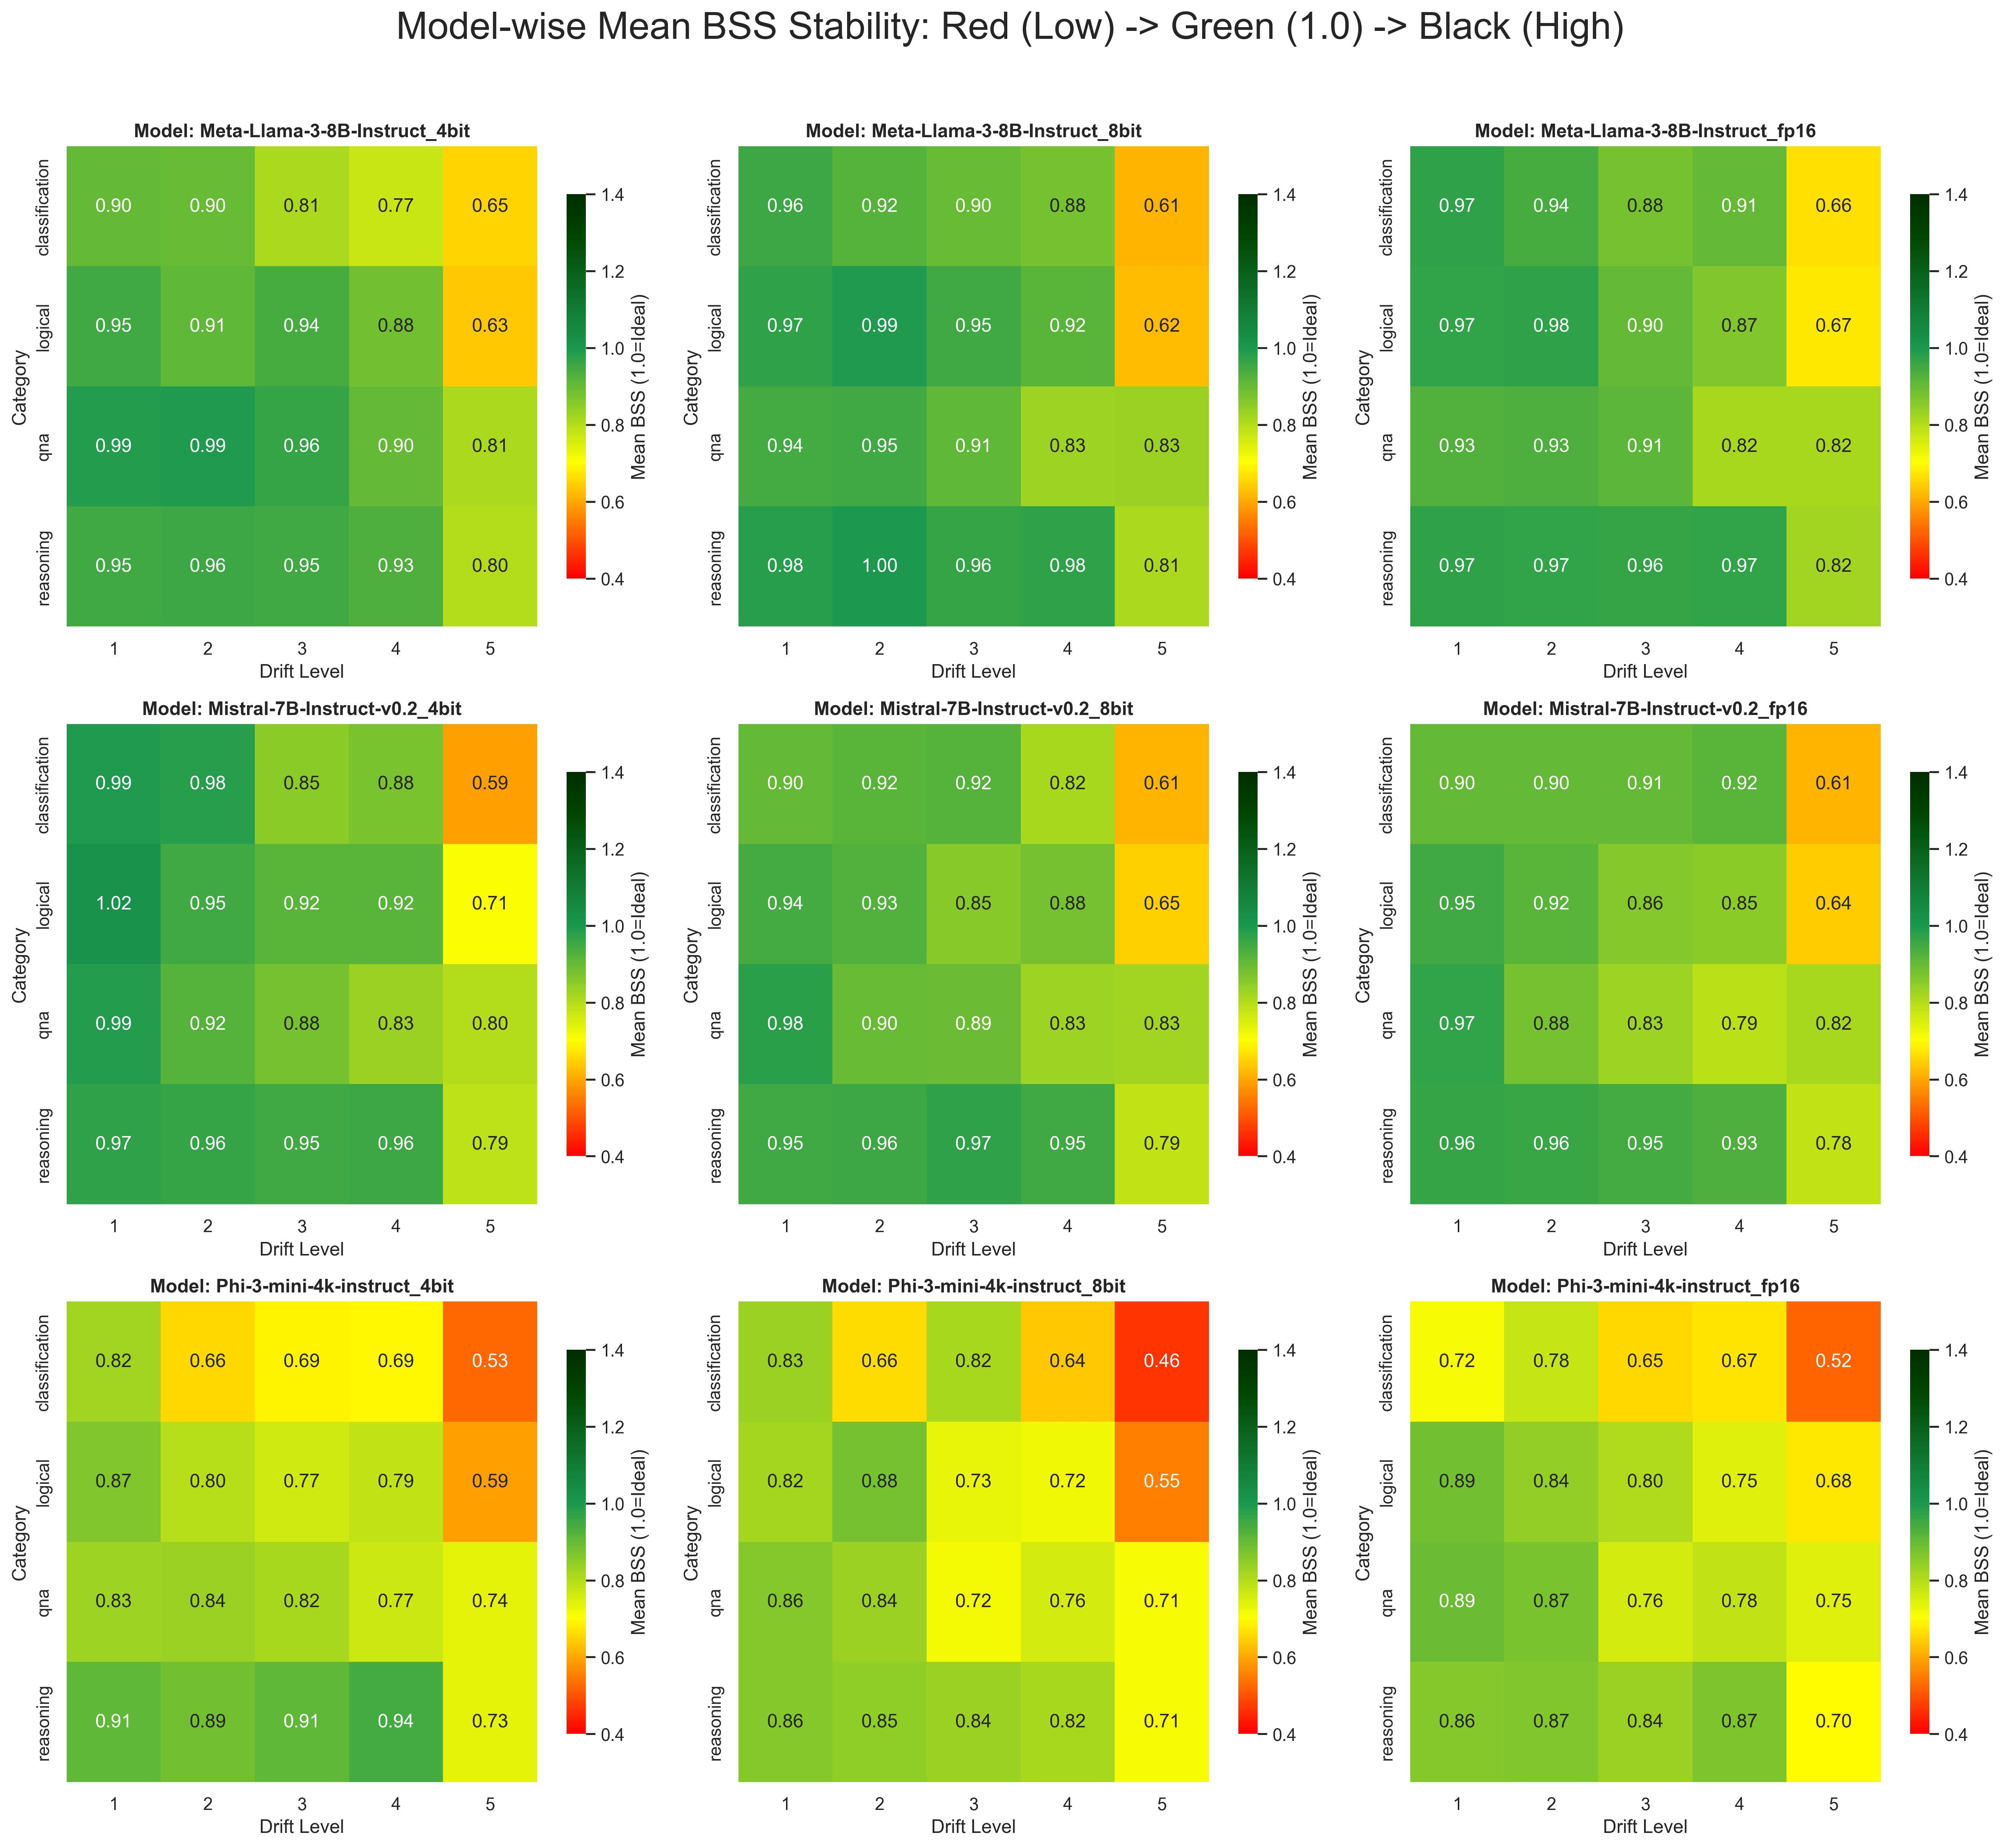
\includegraphics[width=0.85\textwidth]{modelwise_mean_bss.png}
\caption{Model-wise Mean BSS across drift levels. All models exhibit progressive degradation, with INT4 configurations showing early-stage collapse, indicating high sensitivity to prompt drift.}
\label{fig:modelwise_bss}
\end{figure*}

As shown in Fig.~\ref{fig:modelwise_bss}, all models exhibit a gradual degradation in stability as drift increases, with INT4 configurations collapsing significantly earlier.

% --- FIGURE 2 + 3 (SIDE-BY-SIDE) ---
% --- FIGURE 2 + 3 (SIDE-BY-SIDE) ---
\begin{figure*}[t]
\centering
\subfloat[Category-wise BSS]{
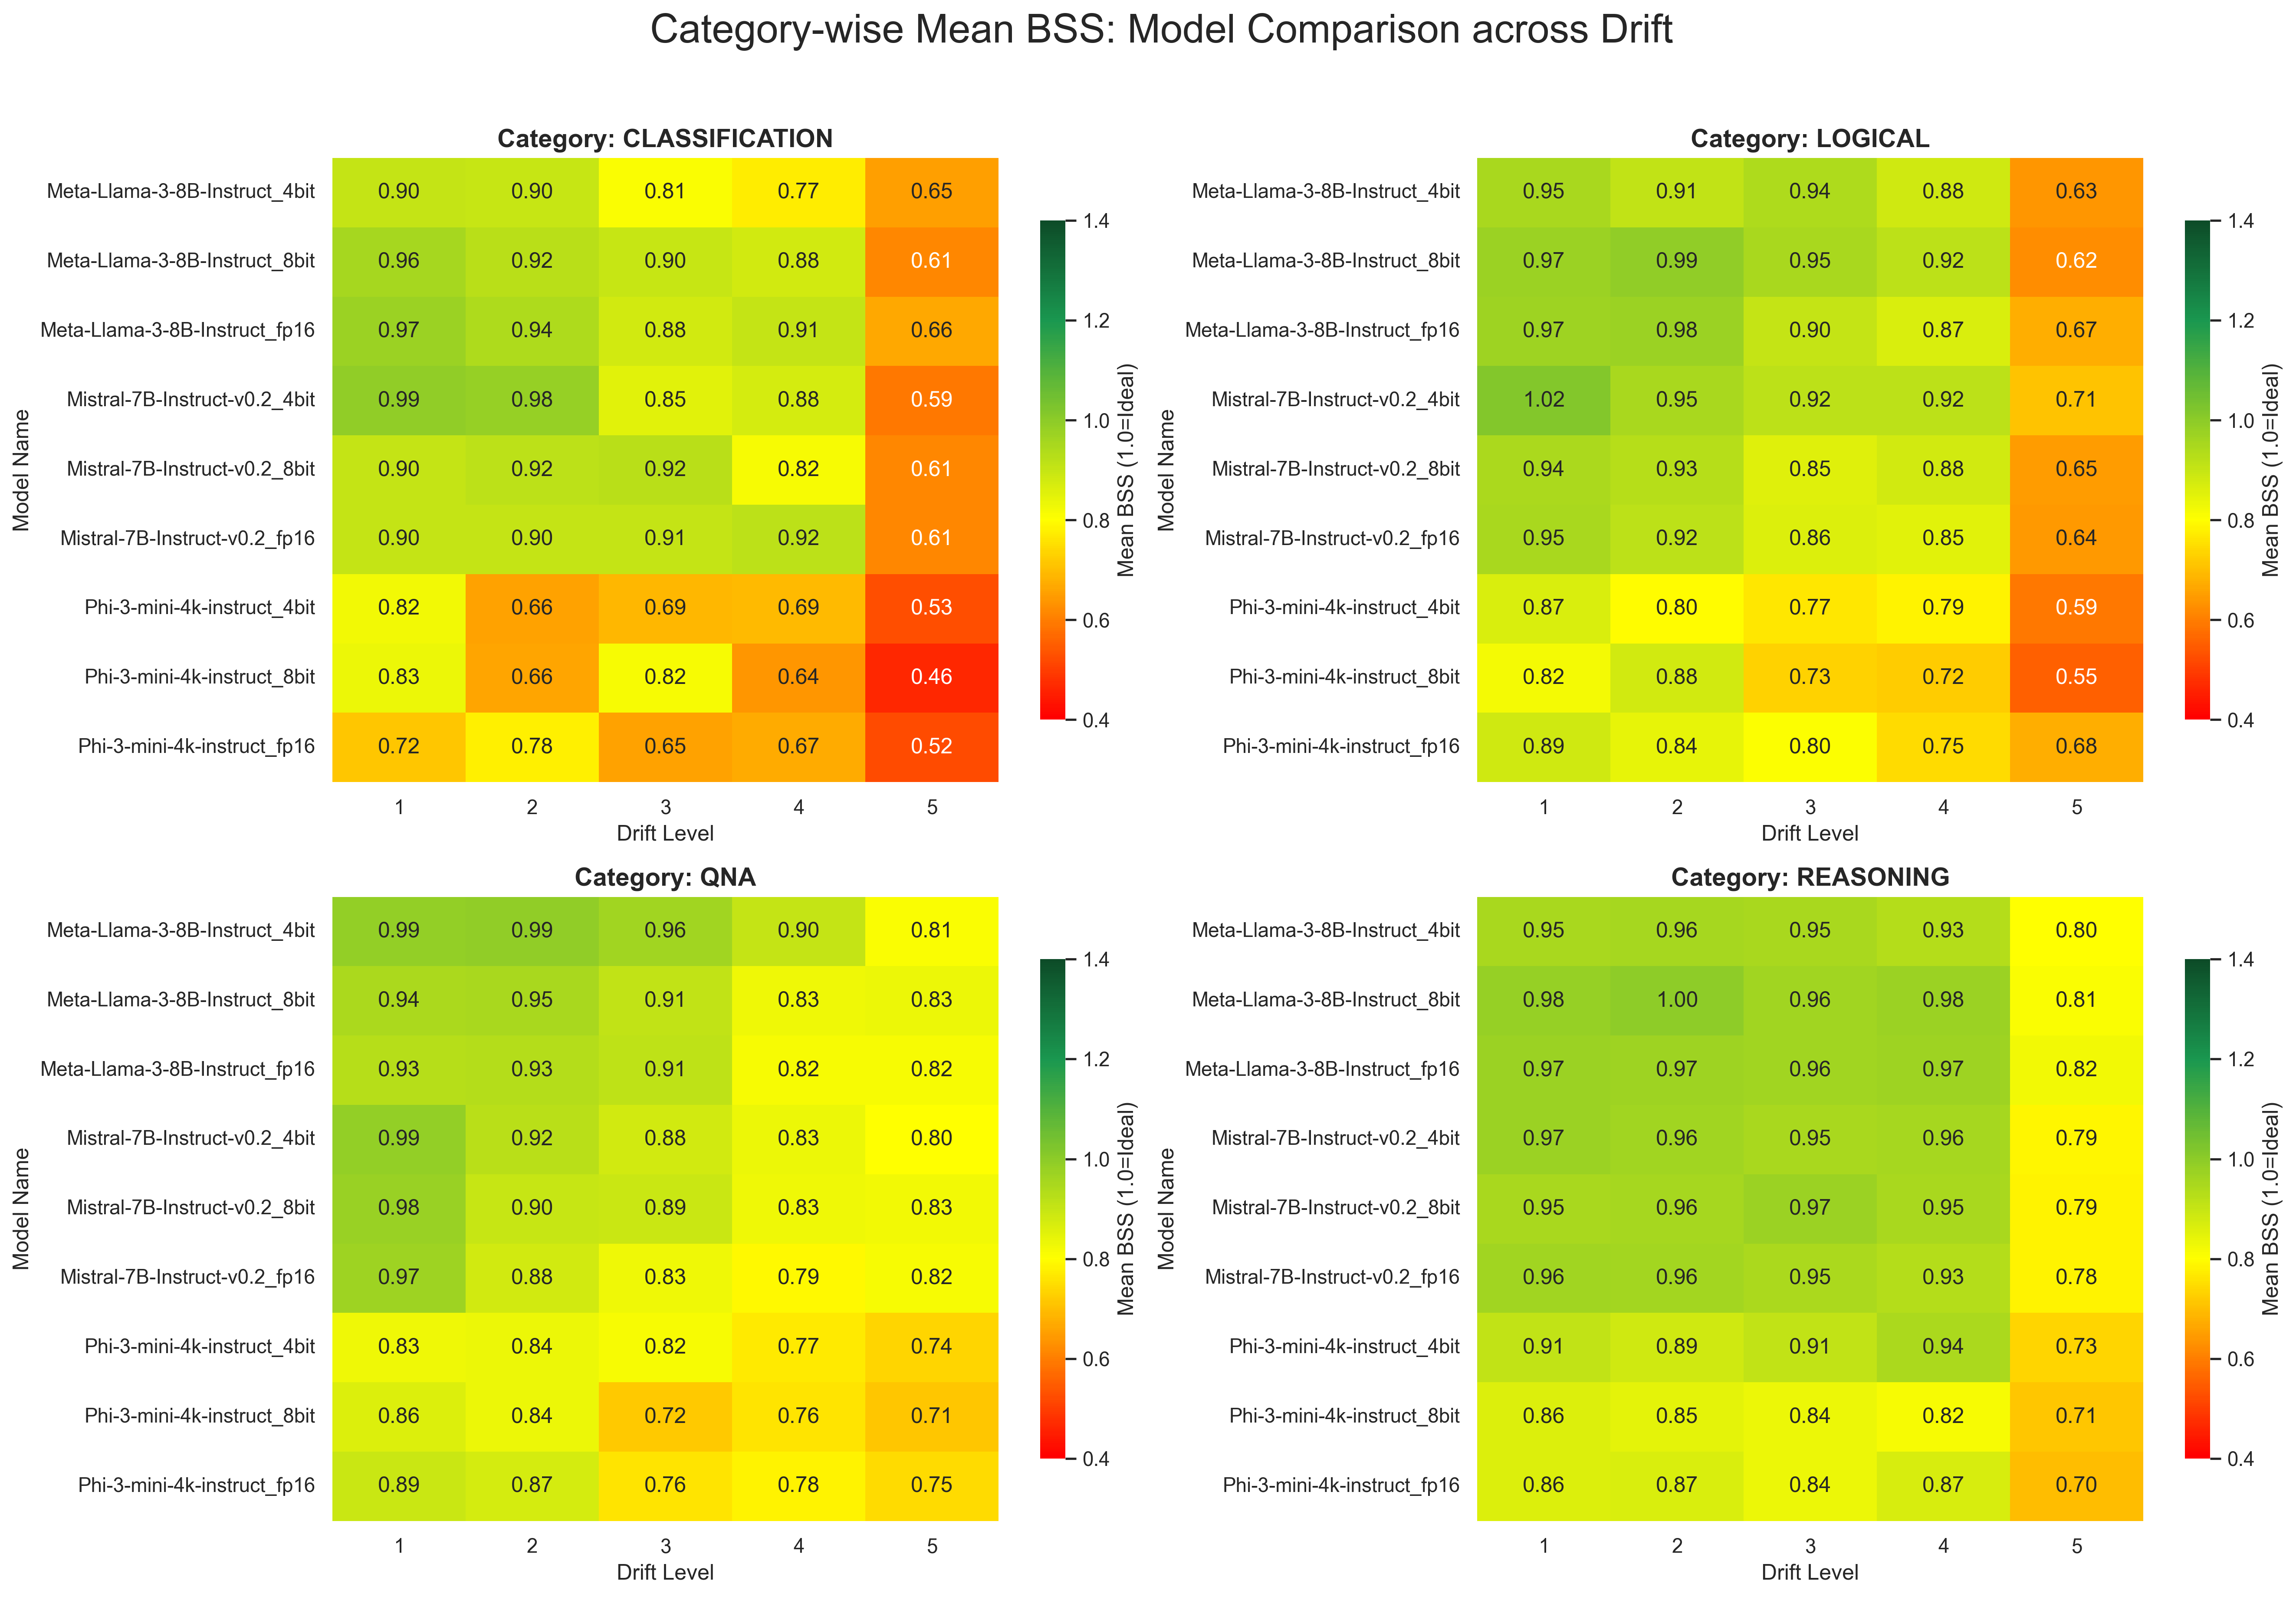
\includegraphics[width=0.45\textwidth]{categorywise_mean_bss.png}
\label{fig:category_bss}
}
\hfill
\subfloat[Aggregated Quantization Impact]{
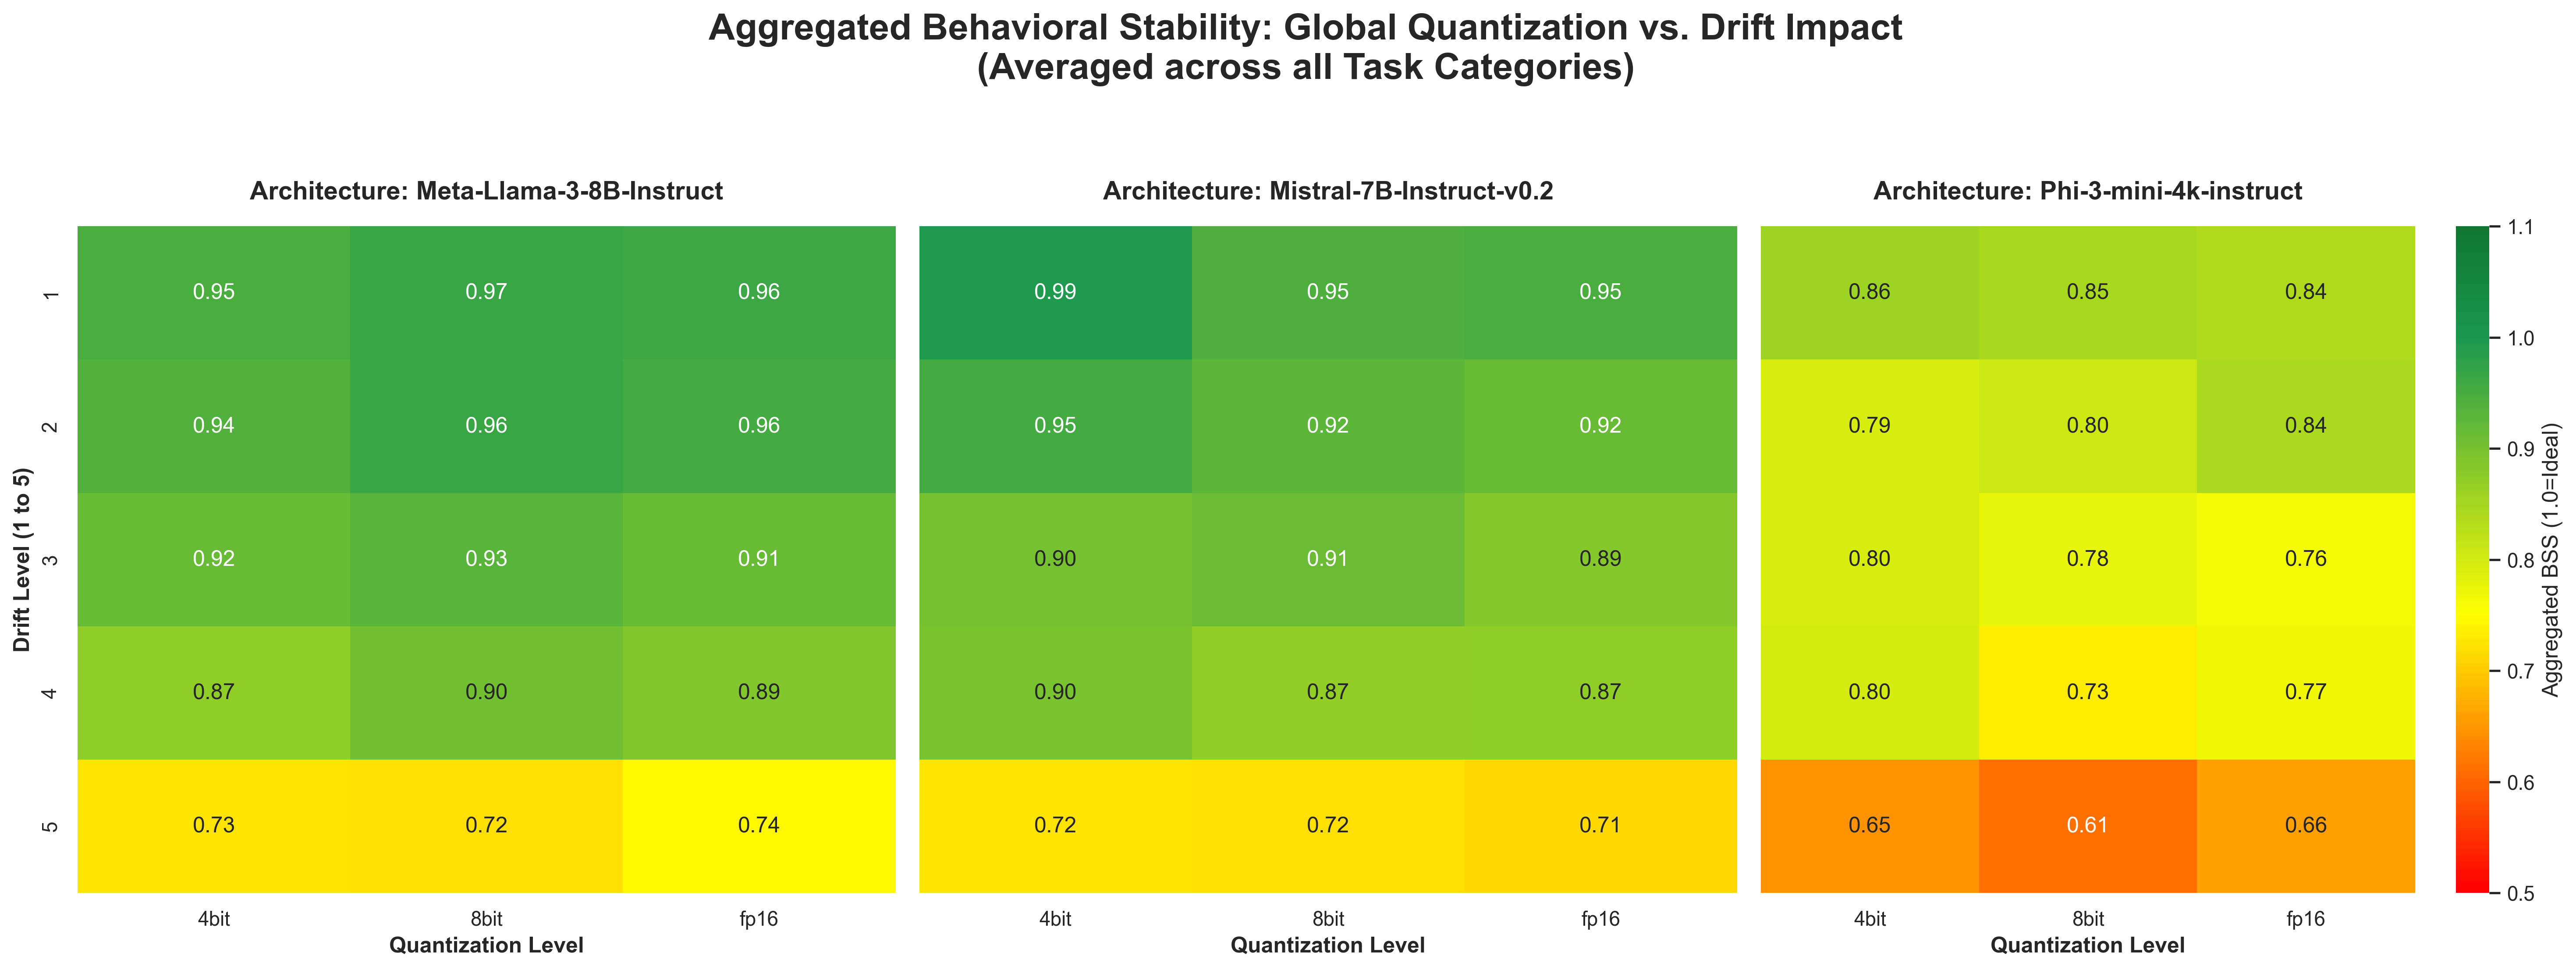
\includegraphics[width=0.45\textwidth]{aggregated_quantization_bss.png}
\label{fig:agg_quant_bss}
}
\caption{(a) Category-wise BSS showing task-dependent robustness differences. (b) Aggregated quantization trends demonstrating a consistent decline in stability with reduced precision.}
\end{figure*}

Fig.~\ref{fig:category_bss}(a) highlights task-specific divergence across categories, while Fig.~\ref{fig:agg_quant_bss}(b) shows the global degradation trend across quantization levels.

% --- FIGURE 4 + 5 (SIDE-BY-SIDE) ---
\begin{figure*}[t]
\centering
\subfloat[Quantization Gap]{
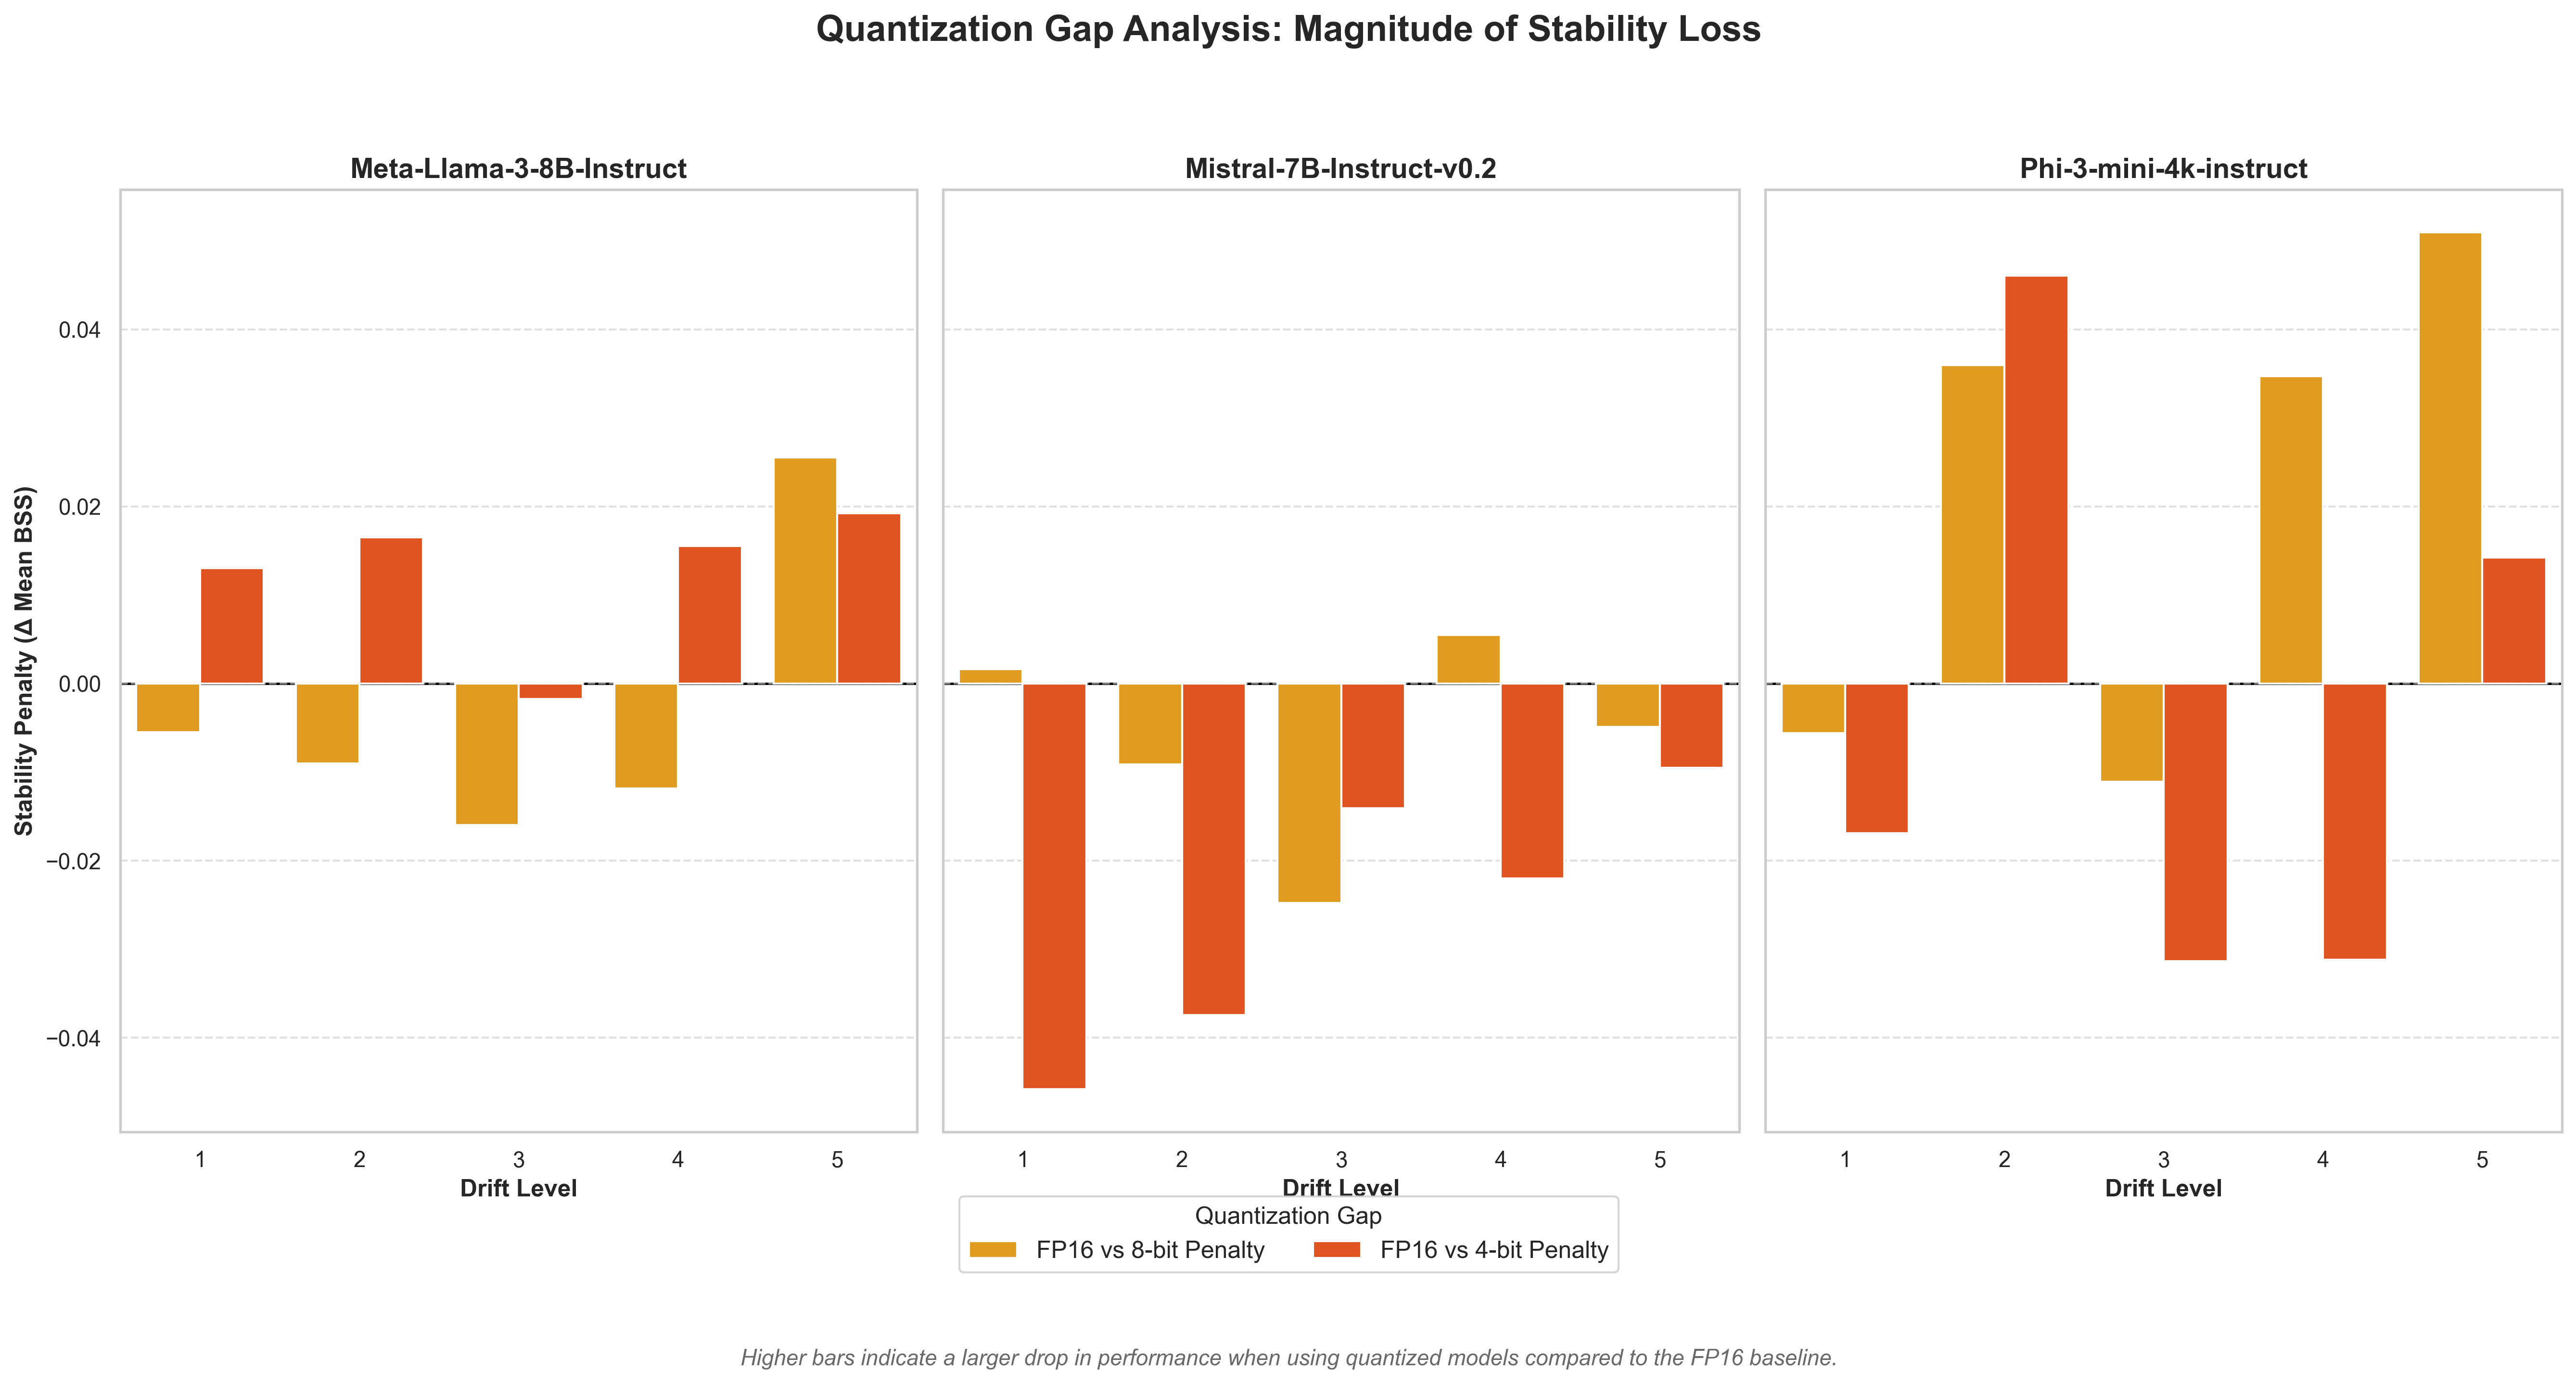
\includegraphics[width=0.45\textwidth]{quantization_gap_analysis.png}
\label{fig:quant_gap}
}
\hfill
\subfloat[Statistical Significance]{
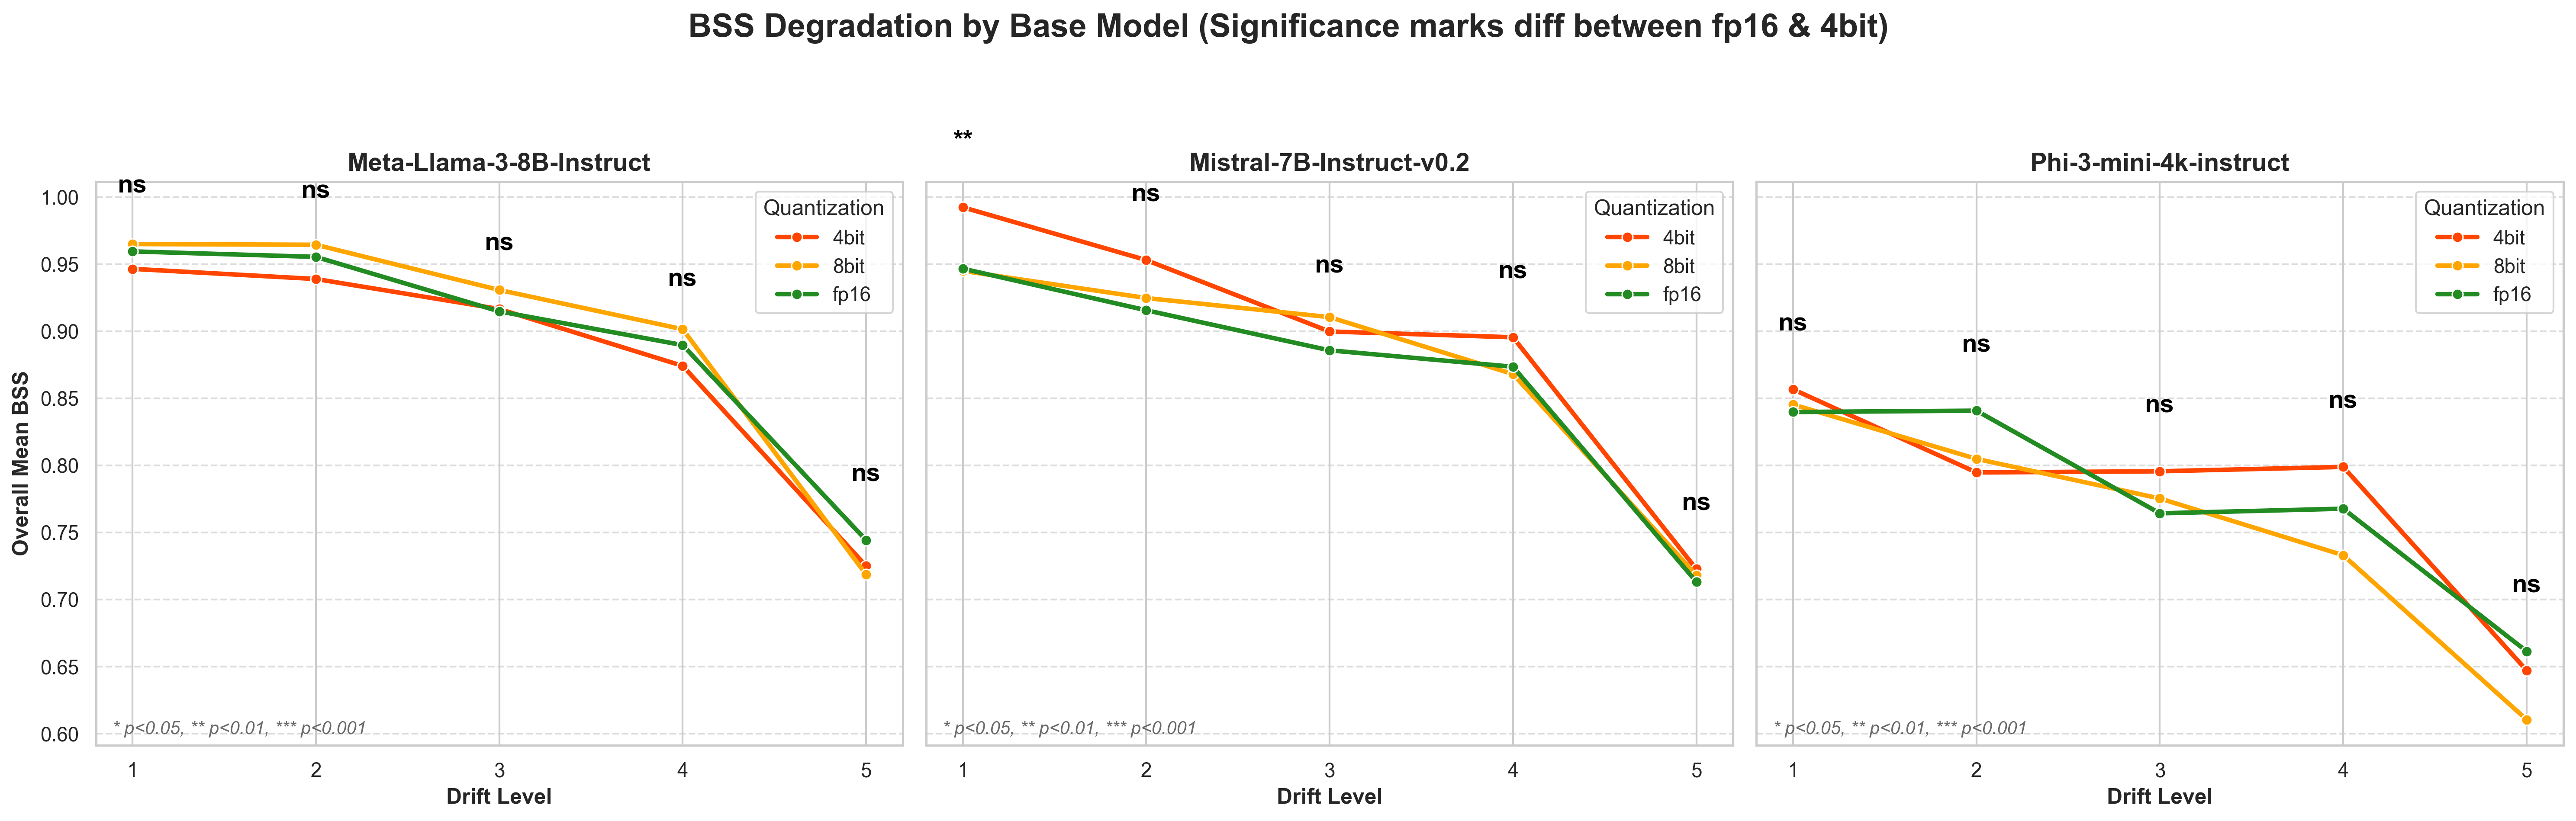
\includegraphics[width=0.45\textwidth]{bss_with_significance.png}
\label{fig:bss_significance}
}
\caption{(a) Quantization gap analysis highlighting disproportionate stability loss in INT4 models. (b) Statistical validation confirming that degradation trends are significant across drift levels.}
\end{figure*}

Fig.~\ref{fig:quant_gap}(a) demonstrates that INT4 degradation is disproportionately higher, while Fig.~\ref{fig:bss_significance}(b) confirms statistical reliability.

% --- FIGURE 6: FINAL INSIGHT (FULL WIDTH) ---
\begin{figure*}[t]
\centering
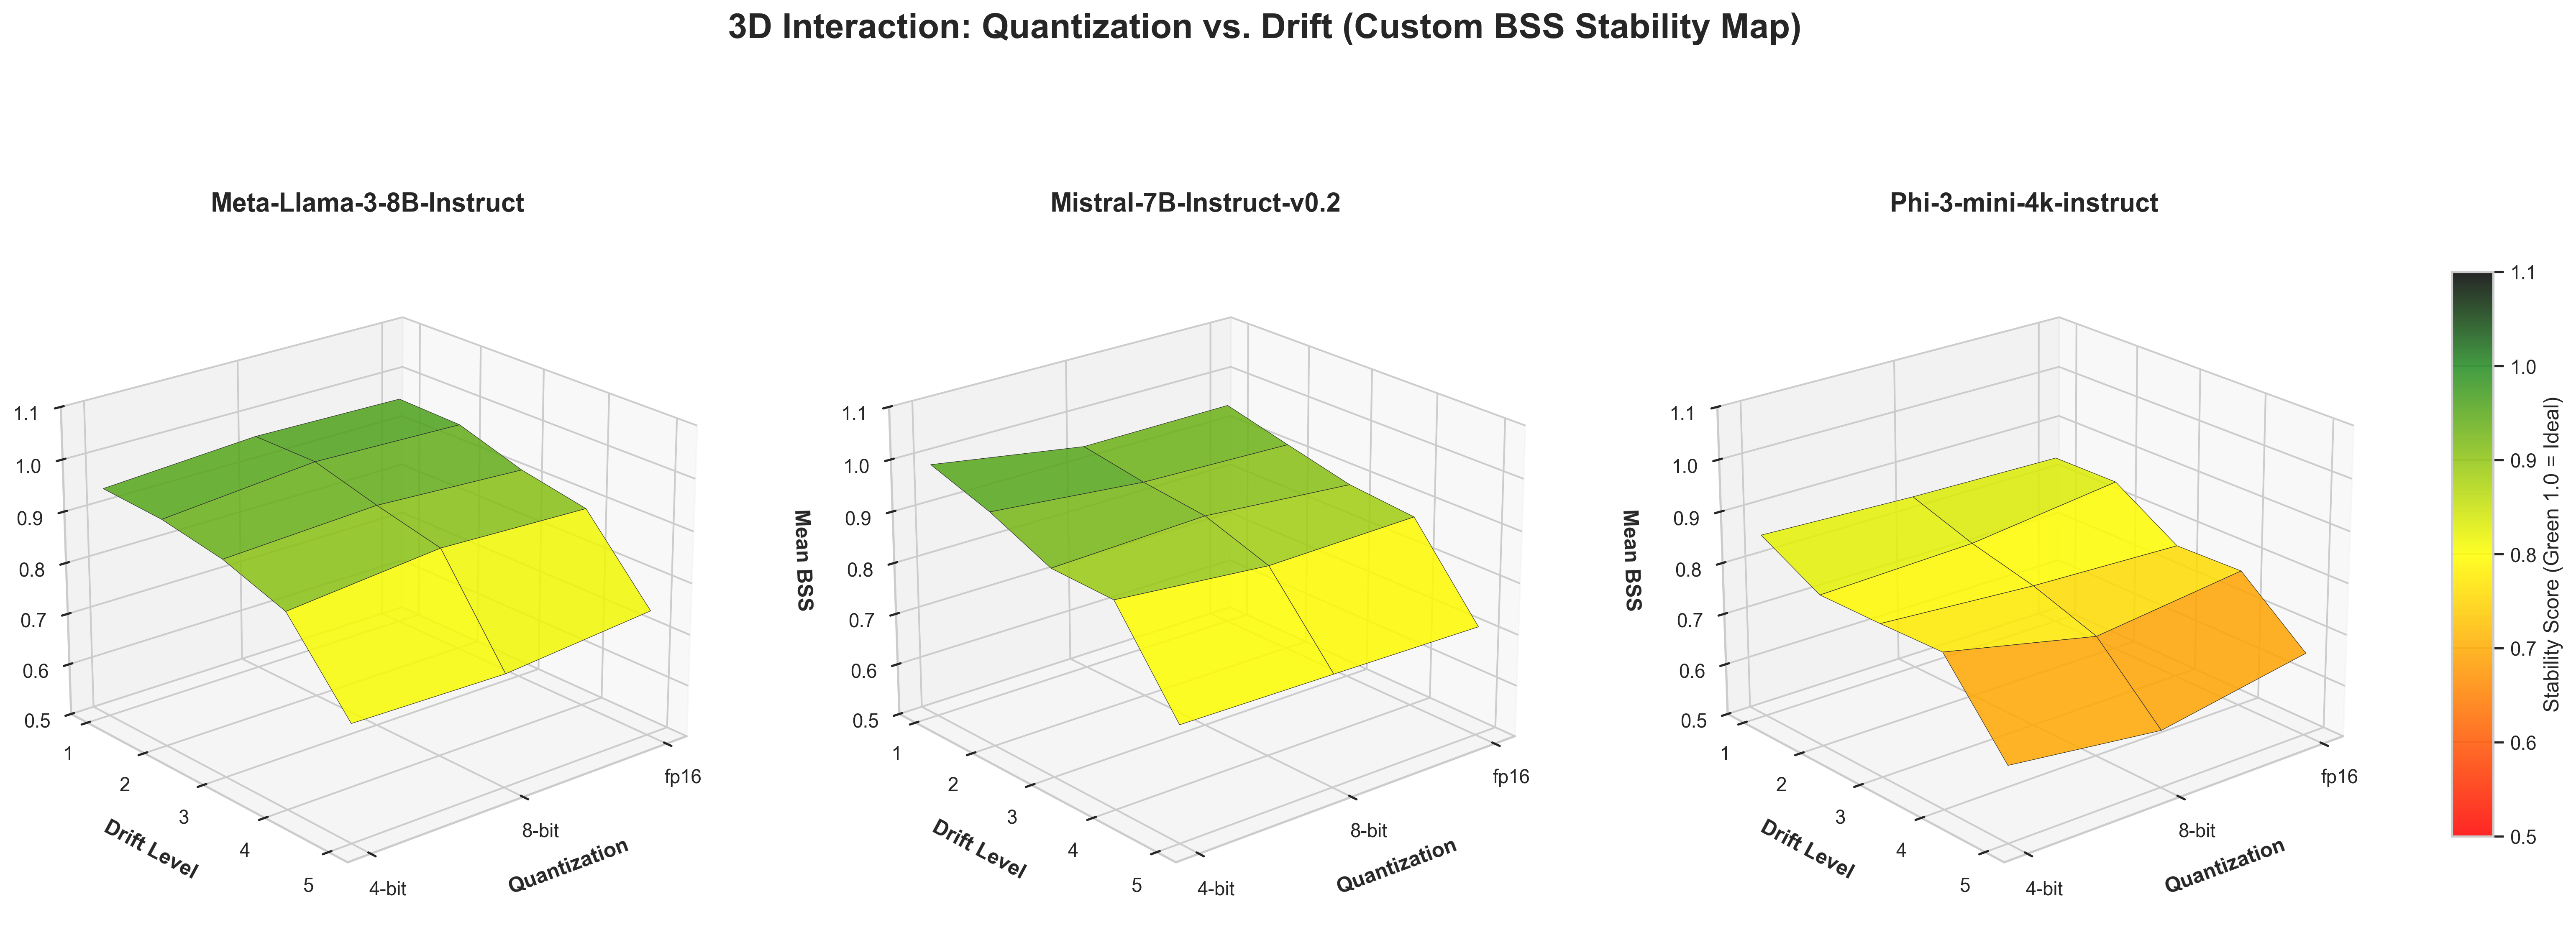
\includegraphics[width=0.85\textwidth]{bss_3d_interaction.png}
\caption{3D interaction between model architecture, quantization level, and drift severity, illustrating the compounded impact of compression and input degradation on behavioral stability.}
\label{fig:bss_3d}
\end{figure*}

Fig.~\ref{fig:bss_3d} illustrates the higher-order interaction between architecture, quantization, and prompt drift.

The empirical analysis of 5,760 model-response pairs uncovers intricate relationships among numerical precision, input quality, and task characteristics. Contrary to initial expectations, the primary finding is that modern quantization techniques demonstrate greater robustness than anticipated, with drift severity emerging as the predominant factor in behavioral degradation.

\subsection{Quantization Impact: Smaller Than Expected }

Our main finding calls into doubt theories regarding quantized model fragility. Compared to FP16 baselines, textit{4-bit quantization adds only 1--3\% more stability loss throughout all examined arrangements}. At drift level 5 (L5), for instance, textit{Llama 3.1 obtains a BSS of 0.74 (FP16) versus 0.73 (4-bit), hence a difference of only 1 percentage point. Likewise, textit{Mistral 7B displays 0.71 (FP16) versus 0.72 (4-bit)}, with 4-bit sometimes surpassing the baseline inside measurement variance.

This modest quantization penalty stands in sharp contrast to the substantial impact of prompt drift itself. \textit{Clean prompts (L0) maintain BSS near 0.95 across all configurations}, while \textit{maximum drift (L5) degrades performance to 0.65--0.74}---a loss of 21--30 percentage points driven primarily by input quality rather than bit precision.

While statistically measurable, the \textit{1--3\% quantization effect suggests that modern compression techniques}---particularly those implemented in \textit{BitsAndBytes}---\textit{successfully preserve the semantic processing capabilities necessary for handling noisy inputs}. This finding indicates that \textit{concerns about quantization-induced fragility may be overstated for current-generation models}.

\subsection{Task-Specific Fragility: Reasoning vs. Classification}

While quantization effects are modest overall, task category analysis reveals differential robustness patterns:

\begin{itemize}
\item \textbf{Classification Resilience:} Sentiment classification tasks stay ($BSS > 0.80$) through drift level 3 at all quantization levels, even 4-bit. The pattern-matching nature of these tasks seems to be less affected by quantization and moderate input degradation. This is probably because they rely on global semantic cues instead of precise token-level processing.

\item \textbf{Reasoning Sensitivity:} Multi-step reasoning tasks exhibit slightly elevated quantization sensitivity, with 4-bit models attaining the $BSS < 0.70$ threshold roughly one drift level sooner than FP16 in certain configurations. But this difference is still small in absolute terms, only 5 to 7 percentage points.

\end{itemize}

These task-specific patterns suggest that deployment decisions should account for workload characteristics, with reasoning-heavy applications warranting more conservative quantization choices despite the overall modest impact.

\subsection{Drift Dominates as Primary Factor}

The most important factor that affects behavioral stability is the quality of the prompt itself. Moving from L1 to L5 drift causes BSS degradation of about 15\% to 35\% across all configurations. This is about 10\% to 15\% larger than the effect of quantization. Even 4-bit models stay stable (BSS $>$ 0.70) up to drift level 3 for most task categories, which is worth noting.

This finding suggests that production deployments should focus on input normalization and quick quality control mechanisms, as these lead to much bigger stability improvements than avoiding quantization.


\subsection{Confidence–Accuracy Considerations under Prompt Drift}

Confidence–accuracy misalignment is a recognized factor in the assessment of large language models. In this study, we find that linguistic fluency, measured by the \textit{Manner of Language (ML)} score, tends to remain stable, whereas other dimensions, including \textit{Factual Correctness (FC)} and \textit{Logical Correctness (LC)}, deteriorate as prompt drift intensifies.

This pattern indicates that models might persist in producing coherent and well-organized responses despite the influence on underlying accuracy. Nonetheless, the current study does not explicitly quantify confidence levels or assess the divergence between confidence and correctness.

Consequently, a comprehensive examination of calibration and associated confidence-related risks remains a significant focus for future endeavors.


\subsection{Confidence-Correctness Patterns}

Multi-factor evaluation shows that Manner of Language (ML) scores, which show how confident a person is, stay pretty stable even when Factual Correctness (FC) and Logical Correctness (LC) go down. This difference between confidence and accuracy can be seen at all levels of precision. However, it is slightly stronger in 4-bit configurations at high drift levels (L4-L5).
This divergence does not indicate the catastrophic "silent failure" pattern initially postulated; however, it suggests that confidence scores should not be regarded as dependable indicators of correctness in production systems, especially for quantized models functioning in high input noise environments.


\subsection{Discussion: Implications for Deployment}

Our central finding challenges assumptions about quantized model fragility. Across all tested configurations, \textit{4-bit quantization introduces only 1--3\% additional stability loss compared to FP16 baselines}. For example, at drift level 5 (L5), \textit{Llama 3.1 achieves a BSS of 0.74 (FP16) versus 0.73 (4-bit)}---a difference of just 1 percentage point. Similarly, \textit{Mistral 7B shows 0.71 (FP16) versus 0.72 (4-bit)}, with 4-bit occasionally outperforming the baseline within measurement variance.

This modest quantization penalty stands in sharp contrast to the substantial impact of prompt drift itself. \textit{Clean prompts (L0) maintain BSS near 0.95 across all configurations}, while \textit{maximum drift (L5) degrades performance to 0.65--0.74}---a loss of 21--30 percentage points driven primarily by input quality rather than bit precision.

While statistically measurable, the \textit{1--3\% quantization effect suggests that modern compression techniques}---particularly those implemented in \textit{BitsAndBytes}---\textit{successfully preserve the semantic processing capabilities necessary for handling noisy inputs}. This finding indicates that \textit{concerns about quantization-induced fragility may be overstated for current-generation models}.



\section{Deployment Guidelines}

Based on observed stability patterns, we provide the following evidence-based deployment recommendations:

\subsection{Deployment Decision Matrix}

\textit{General Applications:} INT4 quantization is viable for most production deployments. The \textit{1--3\% stability penalty is acceptable given substantial memory savings}.

\textit{Reasoning-Heavy Tasks:} INT8 is recommended for complex mathematical or logical reasoning when input quality cannot be guaranteed. \textit{INT4 remains acceptable if input normalization is implemented}.

\textit{Classification \& Simple QA:} \textit{INT4 is fully suitable}, with high robustness observed across all drift levels.

\textit{Safety-Critical Systems:} FP16 is recommended. While quantization penalties are modest, \textit{zero-tolerance error domains should avoid any additional risk factors}.

\begin{table}[t]
\centering
\caption{Deployment Decision Matrix}
\begin{tabular}{|p{2.2cm}|p{2.2cm}|p{3.5cm}|}
\hline
\textbf{Task Category} & \textbf{Precision} & \textbf{Operational Constraint} \\
\hline
Reasoning / Logic & FP16 / INT8 & INT4 viable only if input similarity $> 90\%$ \\
\hline
Fact-Retrieval (QA) & INT8 & Safe for moderate drift; INT4 requires normalization \\
\hline
Classification & INT4 & Robust under high drift conditions \\
\hline
Safety-Critical & FP16 & Avoid quantization to prevent silent failures \\
\hline
\end{tabular}
\end{table}

\subsection{Strategic Recommendations for Practitioners}

\begin{enumerate}
\item \textit{Prioritize Input Quality Over Quantization Avoidance:} Implementing spell-correction, grammar normalization, or input validation provides \textit{10--15$\times$ larger stability improvements} than avoiding quantization.

\item \textit{Select Robust Architectures:} Model family selection shows a larger impact (\textit{10--13 percentage points}) than quantization level (\textit{1--3 points}). Choose architectures with demonstrated robustness.

\item \textit{Monitor Input Quality, Not Just Confidence:} Track cosine similarity between incoming prompts and clean reference distributions. \textit{Confidence scores alone are insufficient reliability indicators}.

\item \textit{Implement Similarity-Based Escalation:} For critical applications, route low-similarity inputs (\textit{$< 80\%$ cosine similarity to clean reference}) to higher-precision models or human review.
\end{enumerate}

% -----------------------------

\section{Conclusion}

This paper presents the Resilio framework, which is designed to systematically evaluate the relationship between model quantization and realistic prompt degradation. Through an vast review of 5{,}760 responses across nine different model quantization settings and five drift levels, we derive empirical data on stability trends in real production and deployment scenarios.

Our primary discovery shows the commonly held beliefs regarding the vulnerability of quantized models: recent 4-bit quantization results in merely an additional \textit{1--3\%} loss of stability compared to FP16 baselines, whereas the prompt drift accounts for a degradation between \textit{15--35\%}t generation of compression methods.

By introducing a multi-factor evaluation approach through the \textit{Task Performance Score (TPS)} and the \textit{Behavioral Stability Score (BSS)}, we show that stability evaluations must go beyond standard accuracy metrics. The gap observed between linguistic fluency and factual and reasoning accuracy—especially in quantized models exposed to significant drift—emphasizes the necessity for assessment frameworks that are adjusted to specific tasks.

Patterns specific to tasks indicate that although the overall effects of quantization are minor, there are varying sensitivities: classification tasks shows strong resilience even at \textit{4-bit precision}, whereas tasks that require intensive reasoning gain from more cautious quantization options. Nonetheless, these distinctions are still minimal when set against the substantial influence of input quality.

The practical takeaway for this  is  optimization for deployment should be  focus on the  input quality management and robust architectural choices rather than only avoiding aggressive quantization. The stability impact of  the input normalization, which is \textit{10--15$\times$} greater than   precision choice, implies that resources for engineering should  must be better allocated towards improving  preprocessing infrastructure rather than maintaining full precision in production systems.

Future research should probe into the factors those contribute to quantization resilience, whether through analysis of attention patterns, studies on degradation at the layer level, or assessments of embedding quality, in order to develop theoretical models that can predict interactions between quantization and drift. furthermore, conducting user studies to validate the BSS threshold of less than \textit{BSS $<$ 0.70} would support deployment guidelines by linking behavioral metrics with genuine user satisfaction.

The Resilio framework offers both a quantifiable measurement system and a collection of firsthand knowledge that facilitate better-informed decisions regarding deployment. By showing that contemporary quantization can preserve behavioral integrity under the realistic noise circumstances, we  can aim to promote broader acceptance of effective LLM deployment strategies without sacrificing reliability.

% -----------------------------

\begin{thebibliography}{99}

\bibitem{ref1} T. Dettmers \textit{et al.}, ``LLM.int8(): 8-bit Matrix Multiplication for Transformers at Scale,'' NeurIPS, 2022.

\bibitem{ref2} Microsoft Research, ``Phi-3 Technical Report: A Highly Capable Language Model Locally on Your Phone,'' arXiv, 2024.

\bibitem{ref3} A. Zhu \textit{et al.}, ``Robustness in Large Language Models: A Survey of Mitigation Strategies and Evaluation Metrics,'' arXiv, 2024.

\bibitem{ref4} ``Llama vs Mistral vs Phi: Open-Source LLM Comparison,'' 2026.

\bibitem{ref5} ``Evaluating Robustness of Large Language Models Against Input Perturbations,'' 2024.

\bibitem{ref6} ``Intra-Prompt Stability in AI Models,'' 2024.

\bibitem{ref7} ``Understanding and Mitigating Data Drift in LLMs,'' 2024.

\bibitem{ref8} ``Evaluation of On-Device LLMs: Quantization and Performance,'' 2024.

\bibitem{ref9} ``Effect of Noise in LLM Training Data,'' 2024.

\bibitem{ref10} ``Quantization-Based Vulnerability Analysis in LLMs,'' 2024.

\bibitem{ref11} ``Fine-Tuning on Noisy Instructions,'' 2024.

\bibitem{ref12} ``Robustness of LLMs to Typographical Noise,'' 2024.

\bibitem{ref13} ``4-bit vs 8-bit Quantization Analysis,'' 2024.

\bibitem{ref14} ``Key Differences in Quantization Methods,'' 2024.

\bibitem{ref15} ``Edge-Aware Framework for Quantized LLMs,'' 2024.

\bibitem{ref16} ``Quantization-Aware Adaptation for LLMs,'' 2024.

\bibitem{ref17} ``Recent Advances in LLM Research,'' 2024.

\bibitem{ref18} ``Phi-3 Model Card,'' 2024.

\bibitem{ref19} ``Lightweight Open Models by Microsoft,'' 2024.

\bibitem{ref20} ``Behavioral Drift Detection in AI Systems,'' 2024.

\bibitem{ref21} ``Survey on Robustness in Large Language Models,'' 2024.

\end{thebibliography}

\end{document}